\section*{Backup slides}
% Experiment 1 result metric
\begin{frame}[c]{\subsecname: Atrous Rates (Visual Comparison)}
  \centering
  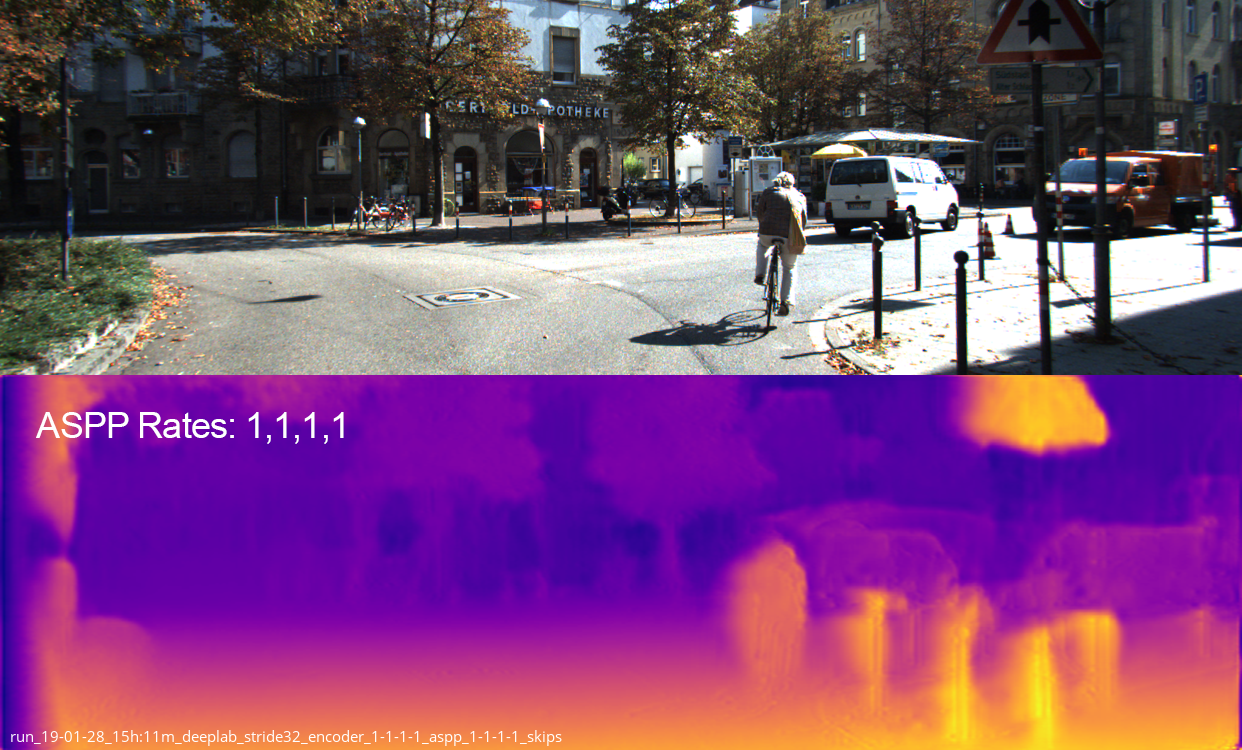
\includegraphics[width=1.0\textwidth]{figures/images/asppcomparison_001.png}
\end{frame}

\begin{frame}[c]{\subsecname: Atrous Rates (Visual Comparison)}
  \centering
  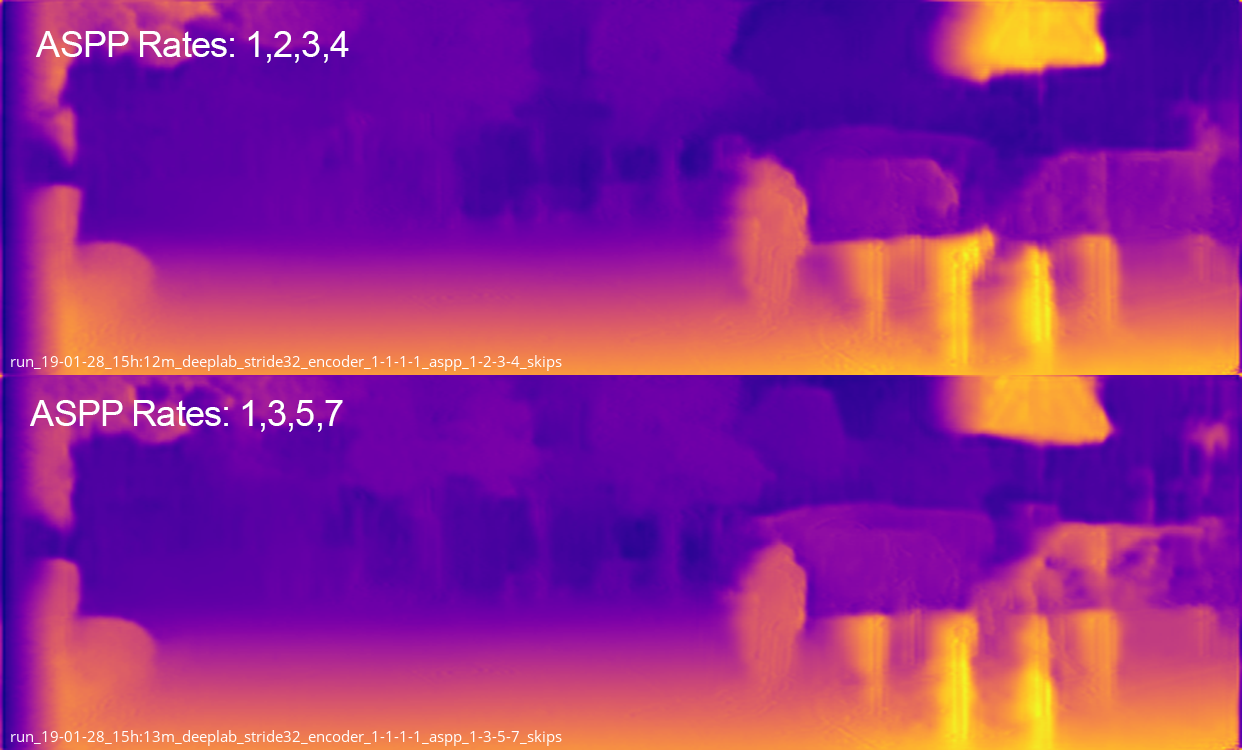
\includegraphics[width=1.0\textwidth]{figures/images/asppcomparison_002.png}
\end{frame}

\begin{frame}[c]{\subsecname: Atrous Rates (Visual Comparison)}
  \centering
  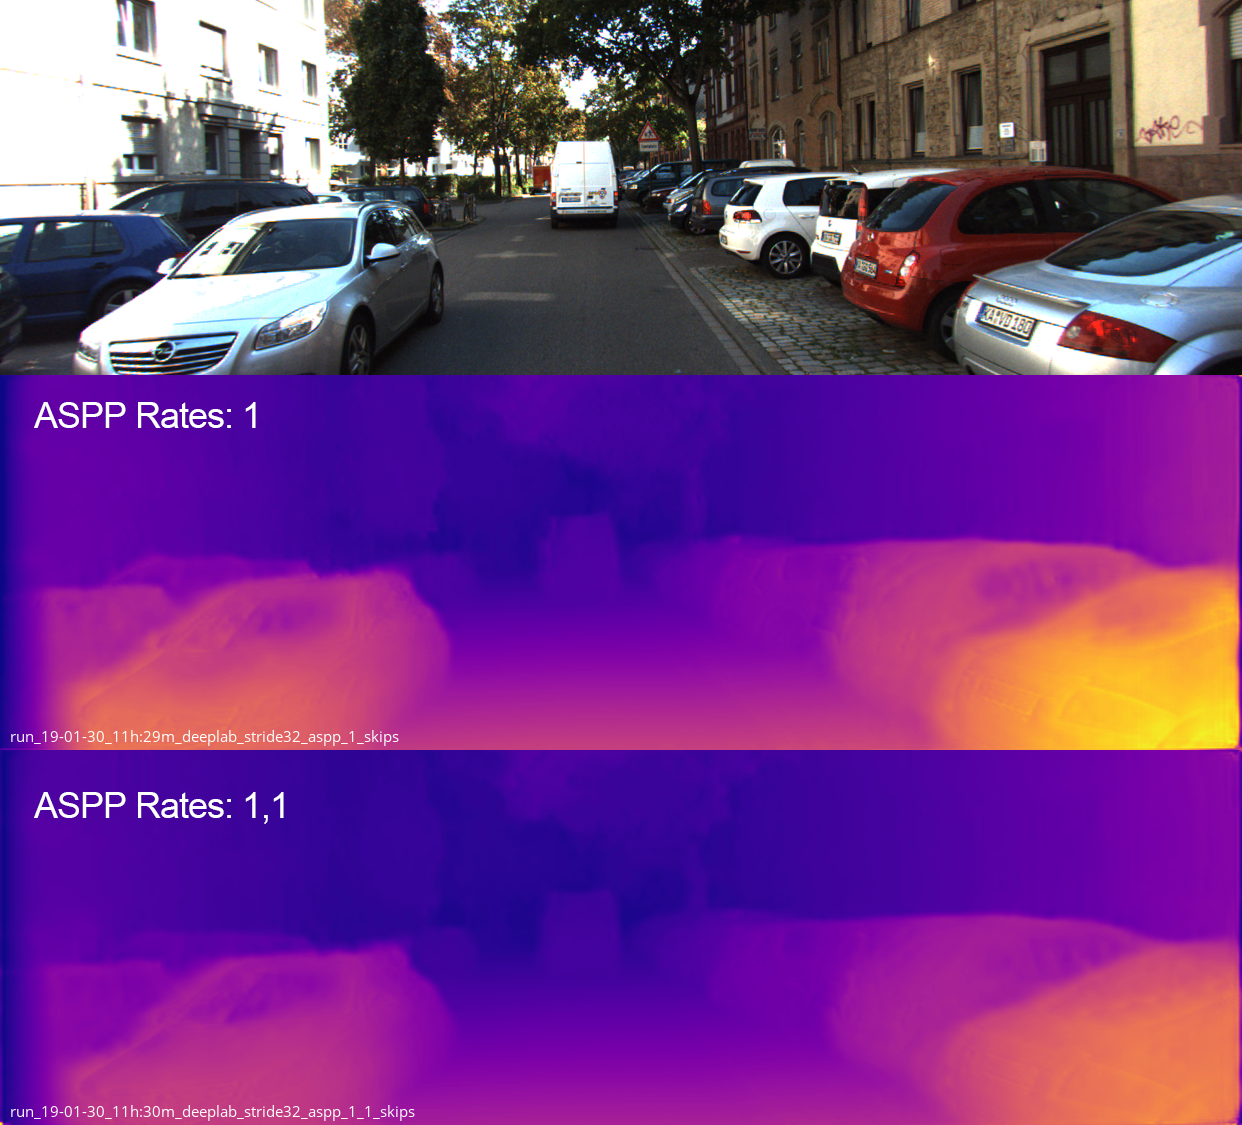
\includegraphics[width=0.7\textwidth]{figures/images/asppconvcomparison_001.png}
\end{frame}

\begin{frame}[c]{\subsecname: Atrous Rates (Visual Comparison)}
  \centering
  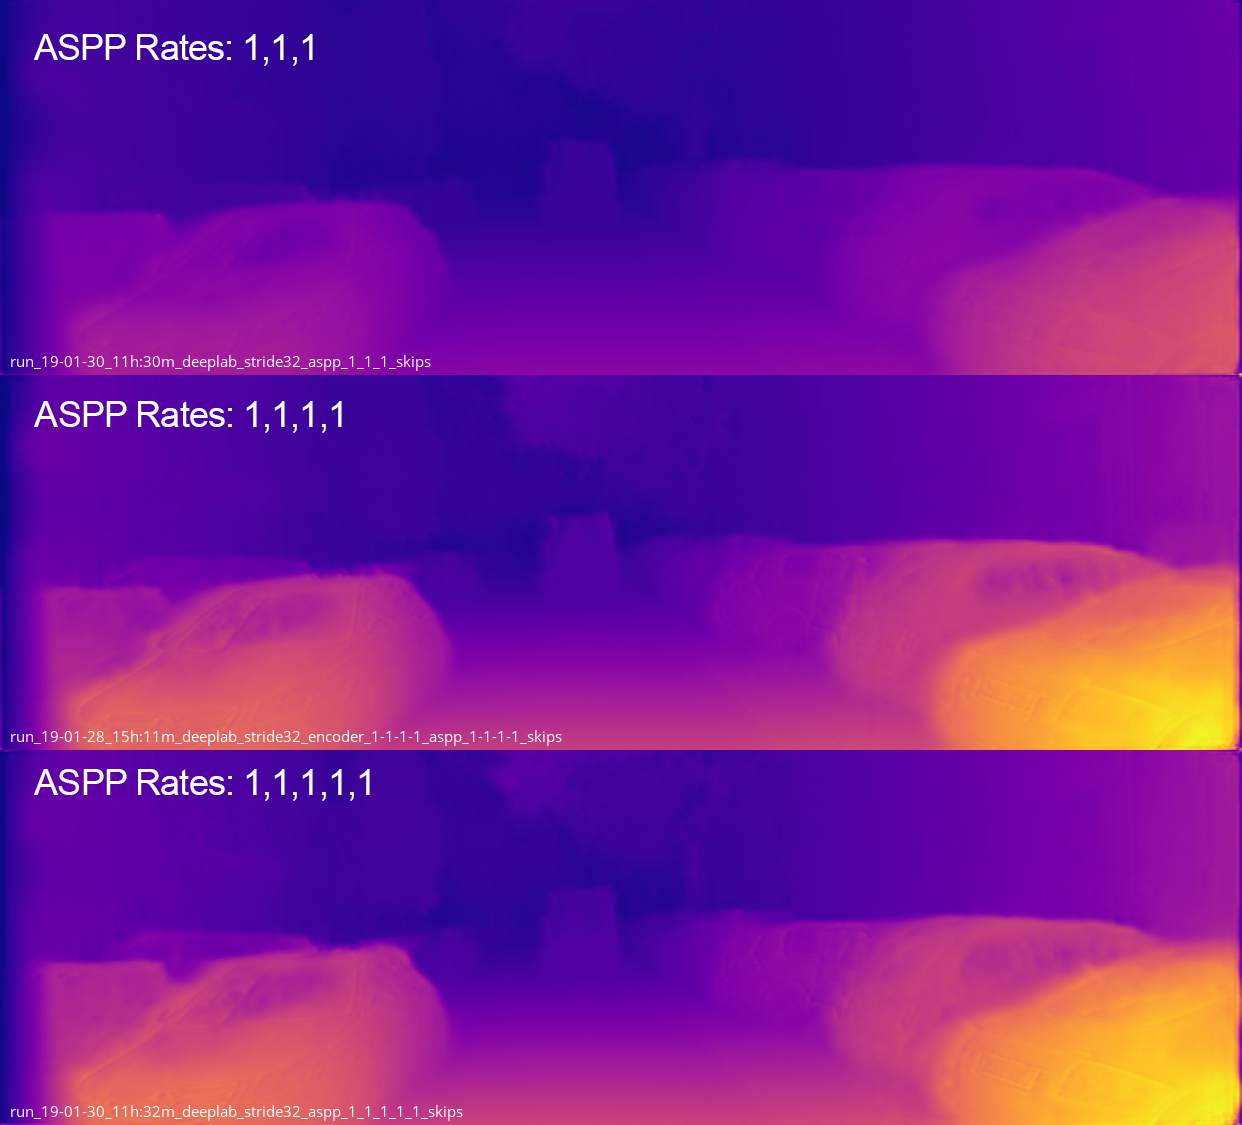
\includegraphics[width=0.7\textwidth]{figures/images/asppconvcomparison_002.png}
\end{frame}



\begin{frame}[c]{\subsecname: Atrous Rates (Squared relative error)}
  \centering
  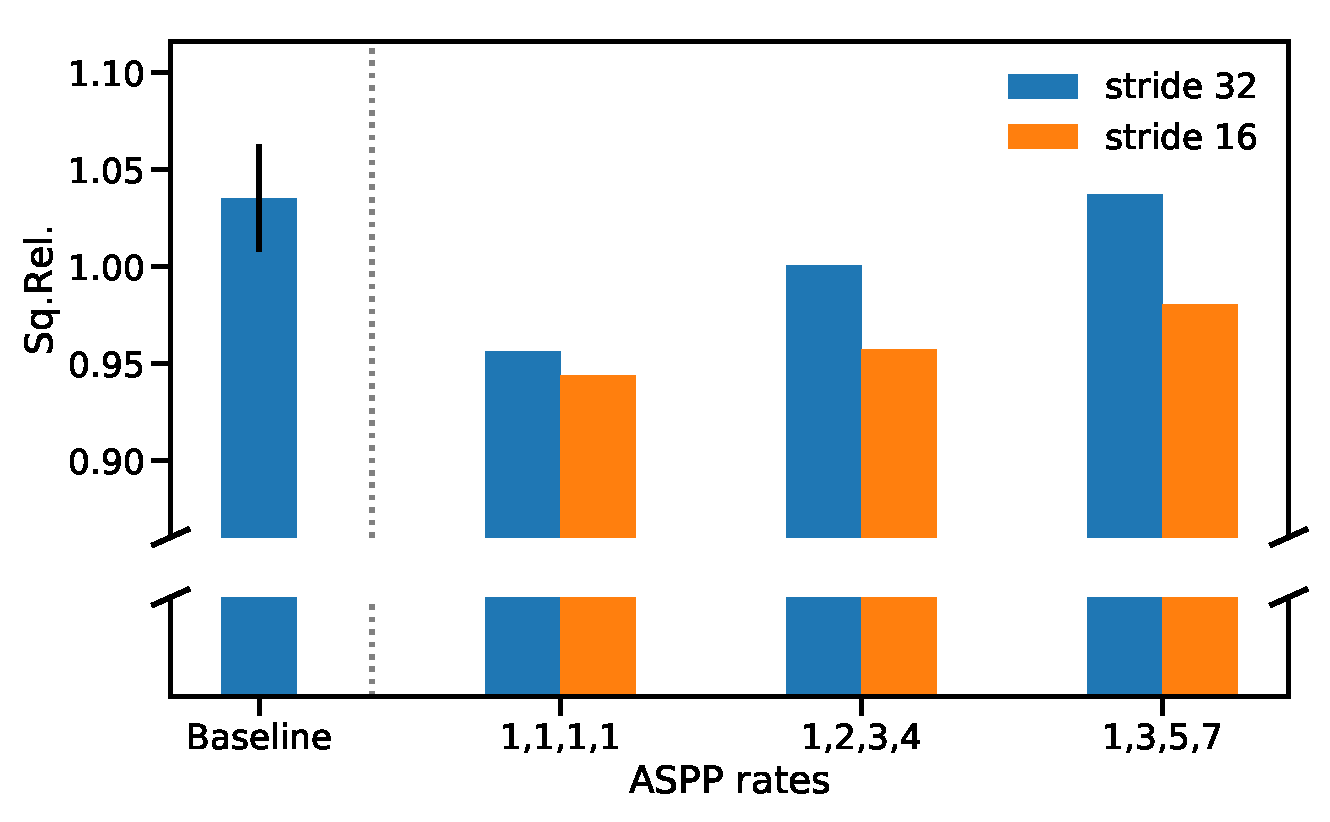
\includegraphics[width=1.0\textwidth]{figures/results/experiment1_SqRel.pdf}
\end{frame}

\begin{frame}[c]{\subsecname: Atrous Rates (RMSE)}
  \centering
  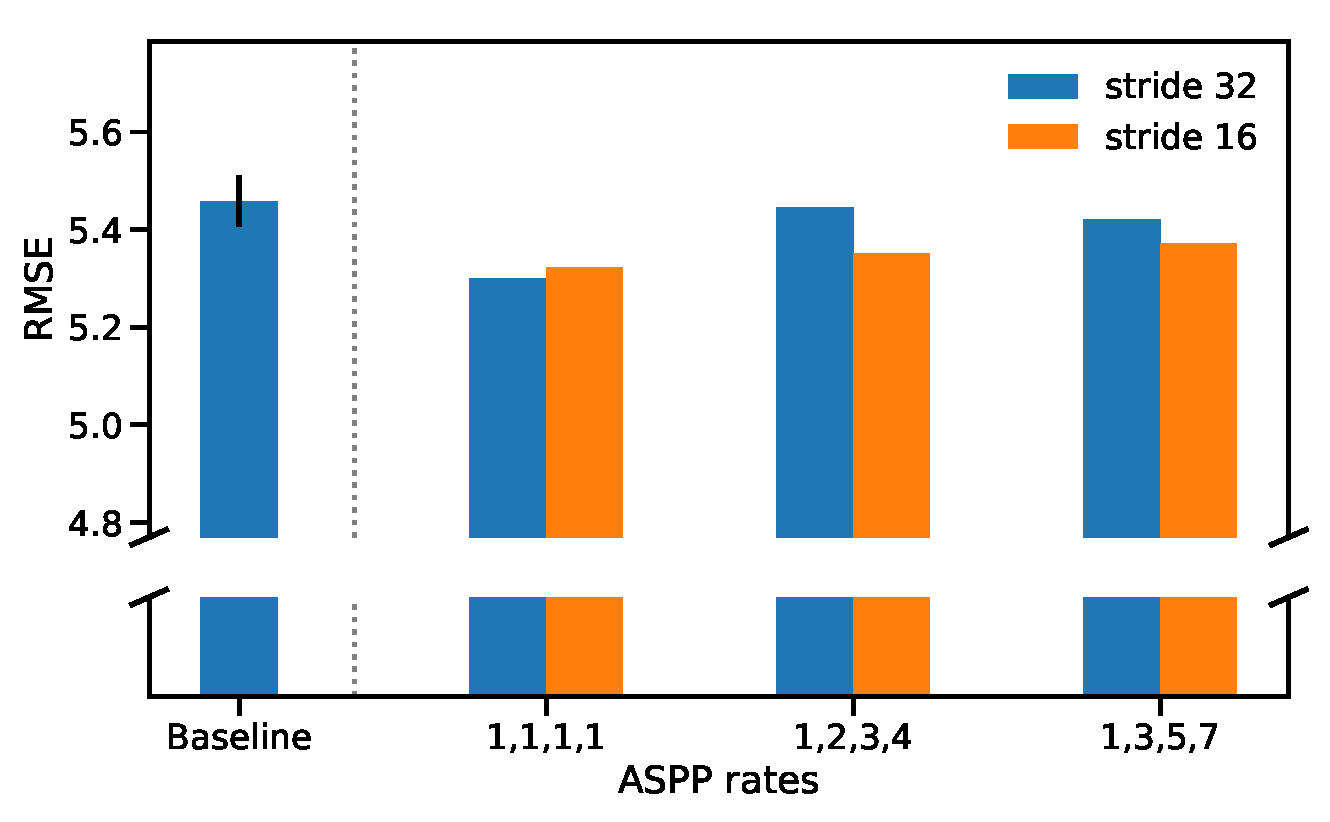
\includegraphics[width=1.0\textwidth]{figures/results/experiment1_RMSE.pdf}
\end{frame}

\begin{frame}[c]{\subsecname: Atrous Rates (RMSE of log)}
  \centering
  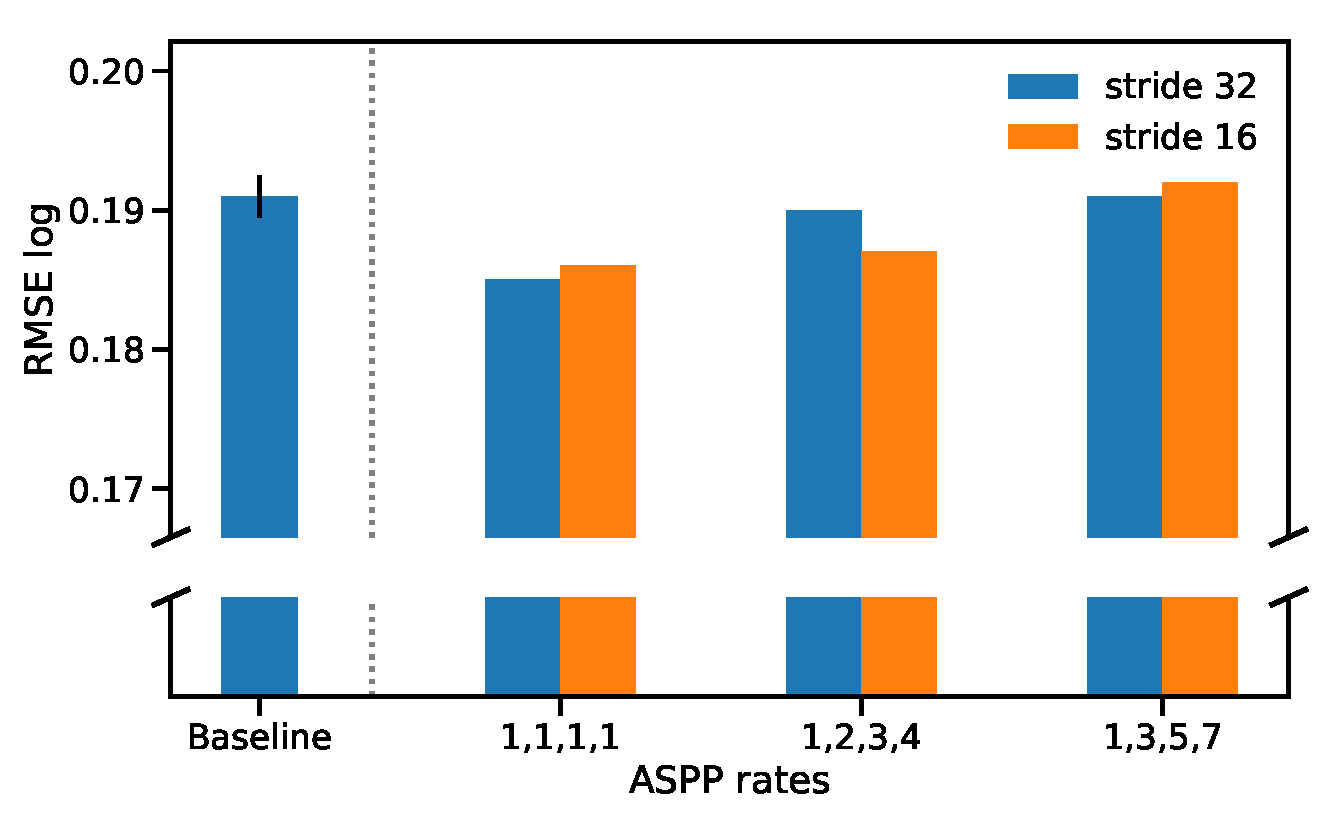
\includegraphics[width=1.0\textwidth]{{figures/results/experiment1_RMSE log}.pdf}
\end{frame}

\begin{frame}[c]{\subsecname: Atrous Rates (\% inliers 1)}
  \centering
  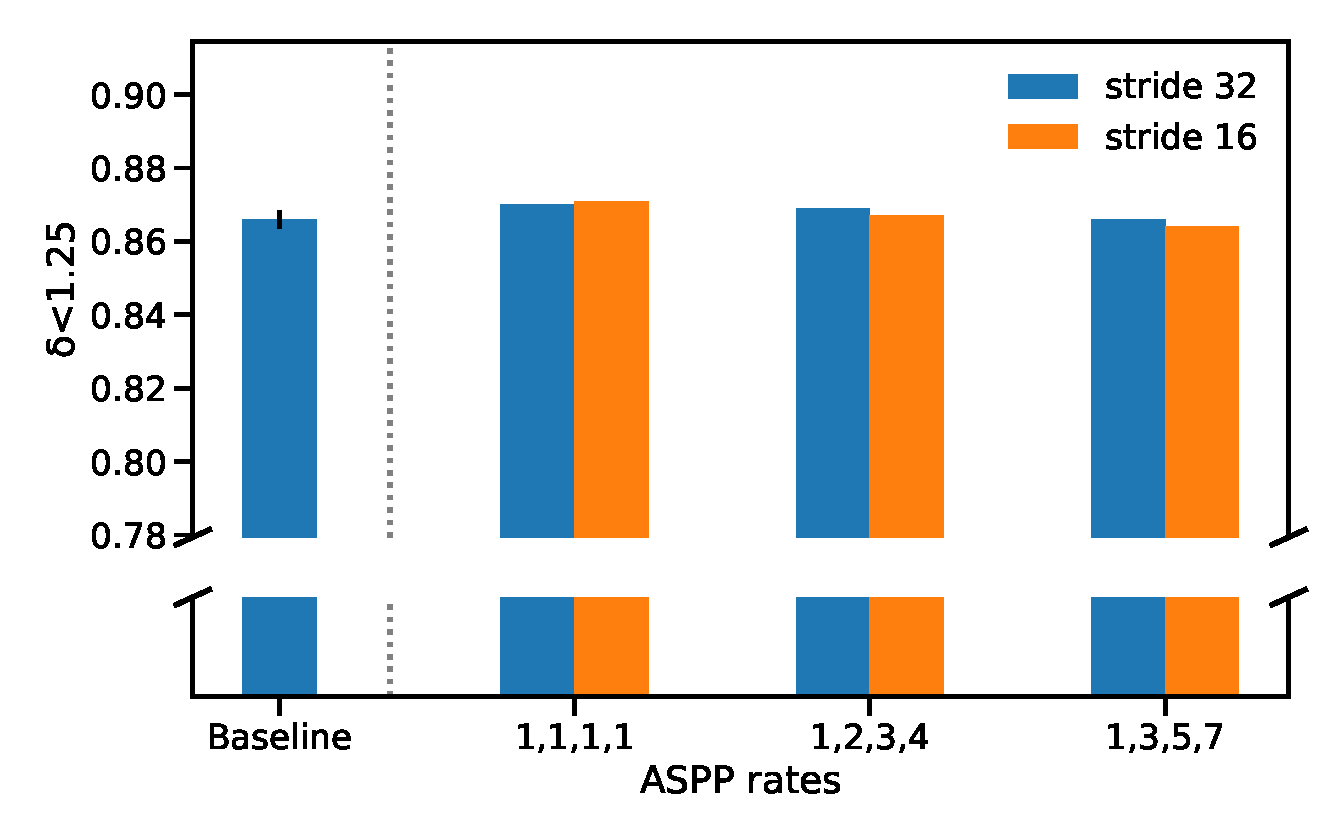
\includegraphics[width=1.0\textwidth]{{figures/results/experiment1_d<125}.pdf}
\end{frame}

\begin{frame}[c]{\subsecname: Atrous Rates (\% inliers 2)}
  \centering
  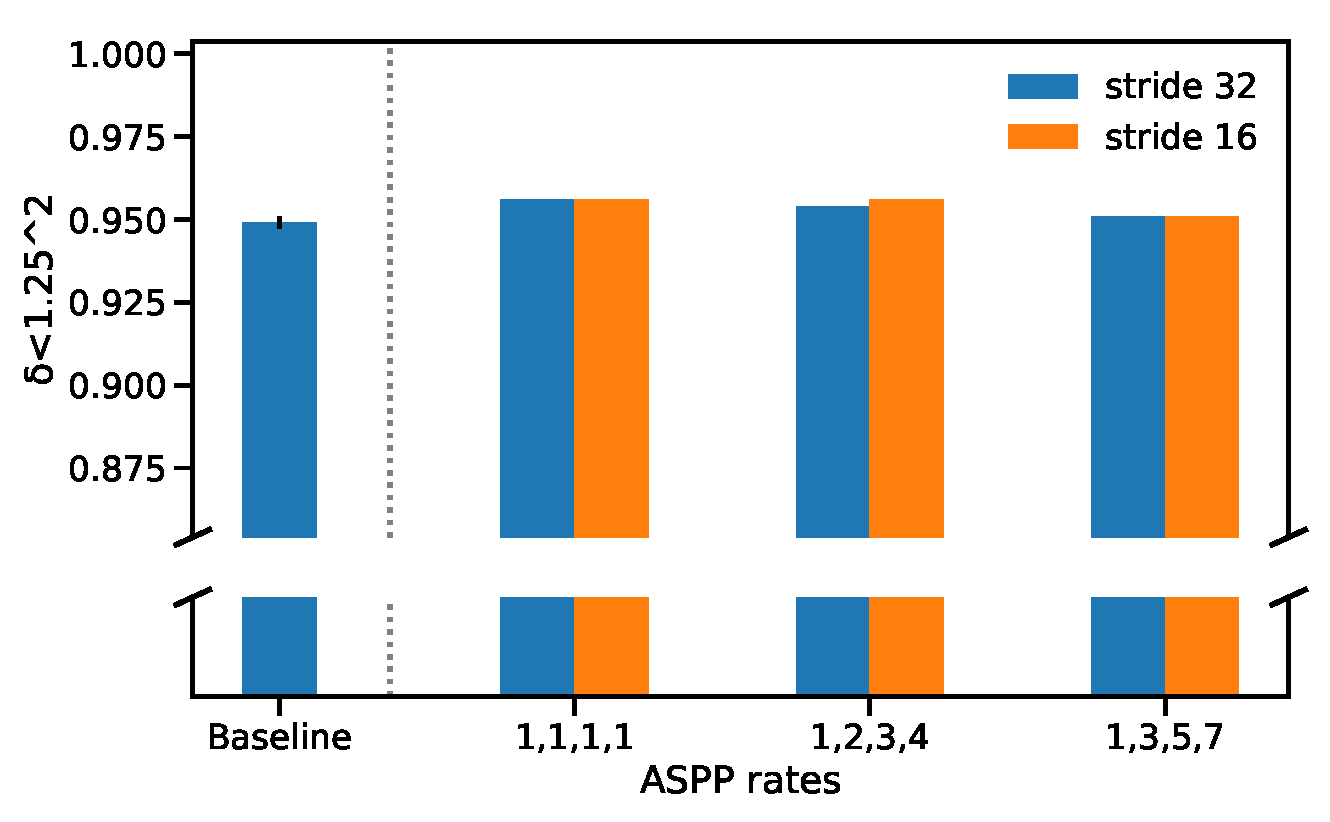
\includegraphics[width=1.0\textwidth]{figures/results/experiment1_d<125^2.pdf}
\end{frame}

\begin{frame}[c]{\subsecname: Atrous Rates (\% inliers 3)}
  \centering
  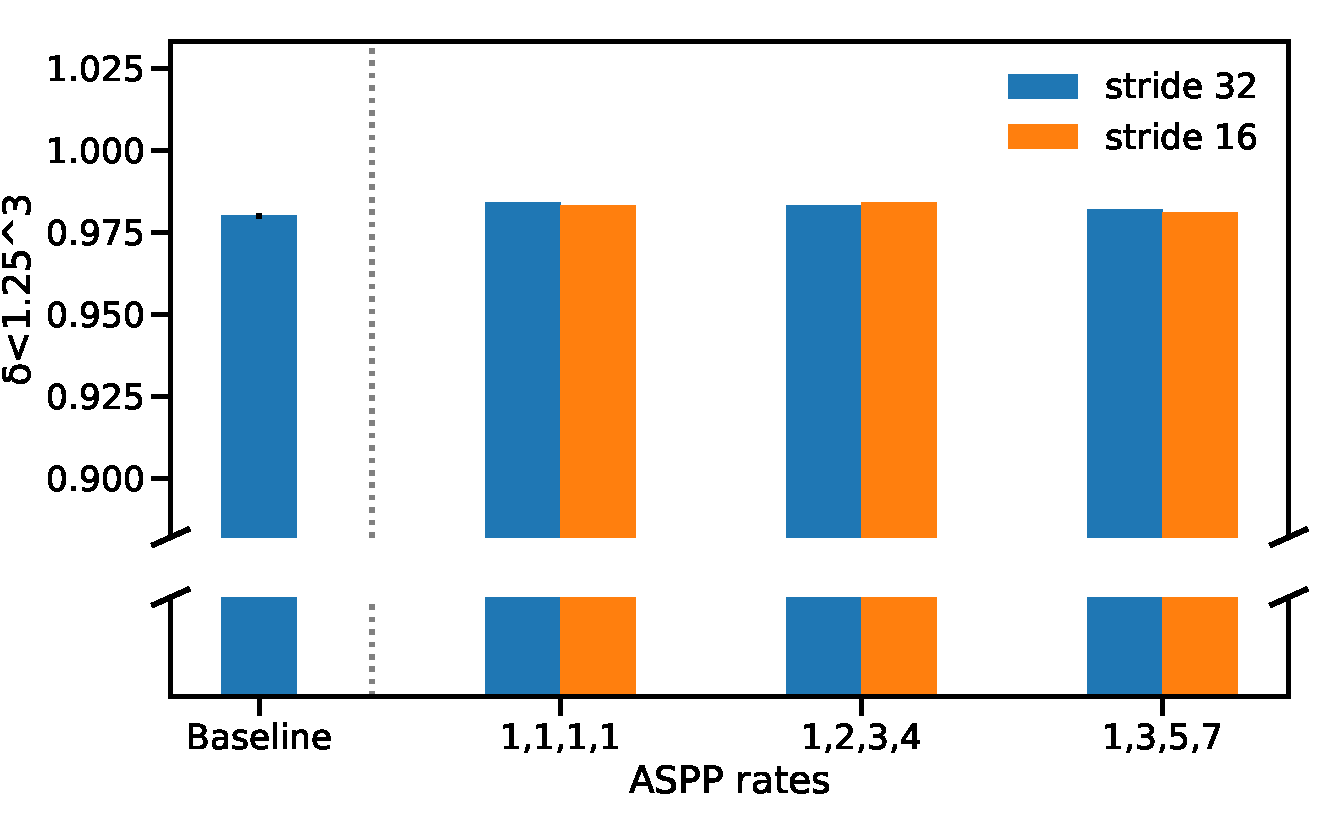
\includegraphics[width=1.0\textwidth]{figures/results/experiment1_d<125^3.pdf}
\end{frame}

\begin{frame}[c]{\subsecname: Atrous Rates (Squared relative error)}
  \centering
  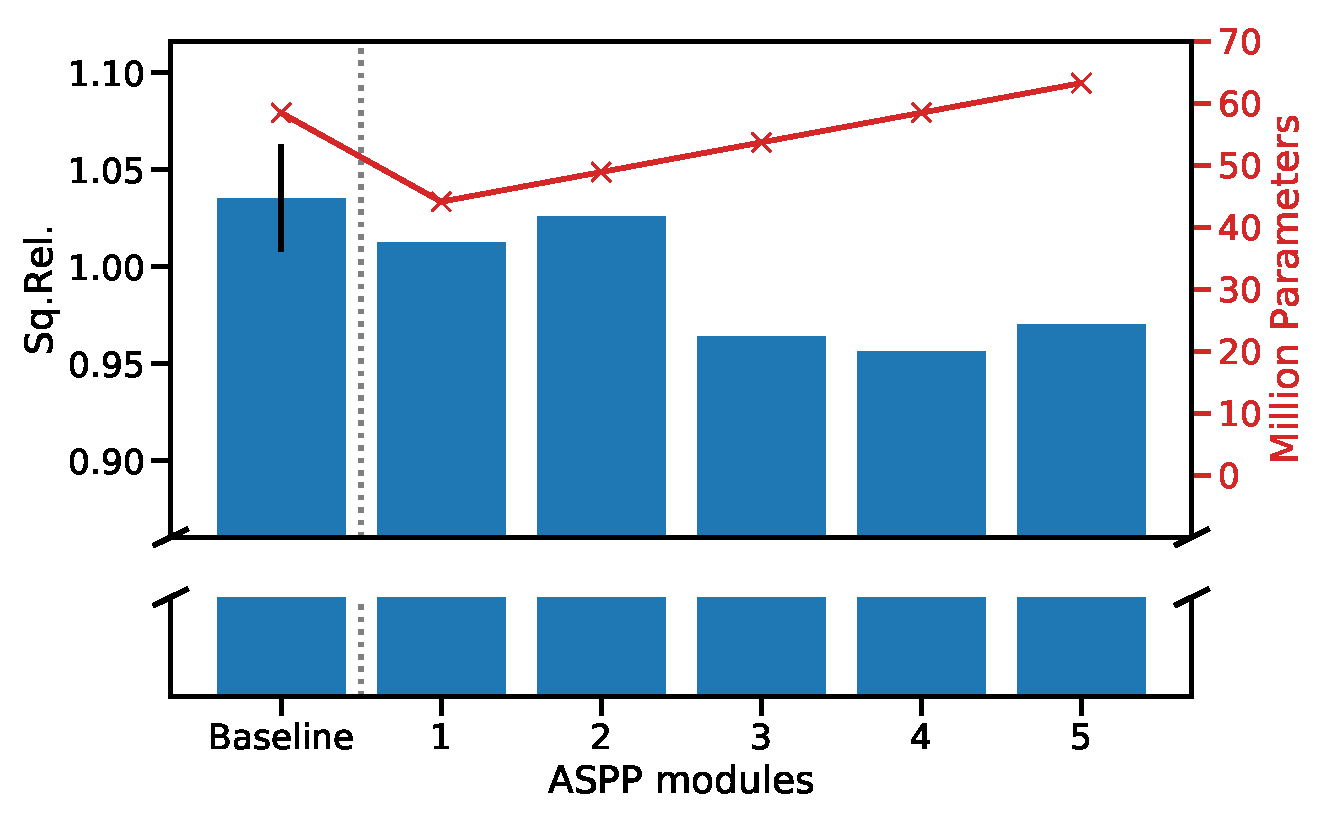
\includegraphics[width=1.0\textwidth]{figures/results/experiment2_SqRel.pdf}
\end{frame}

\begin{frame}[c]{\subsecname: Atrous Rates (RMSE)}
  \centering
  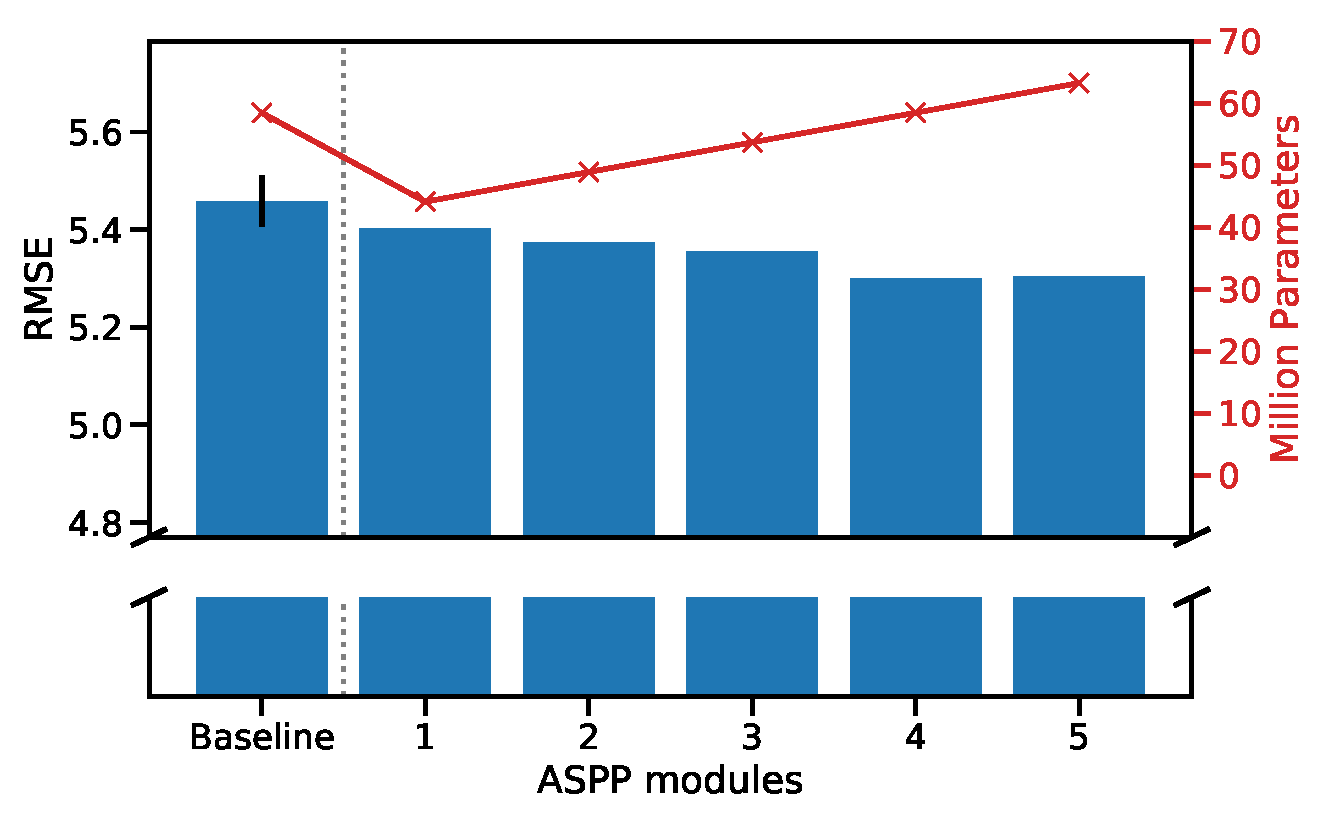
\includegraphics[width=1.0\textwidth]{figures/results/experiment2_RMSE.pdf}
\end{frame}

\begin{frame}[c]{\subsecname: Atrous Rates (RMSE of log)}
  \centering
  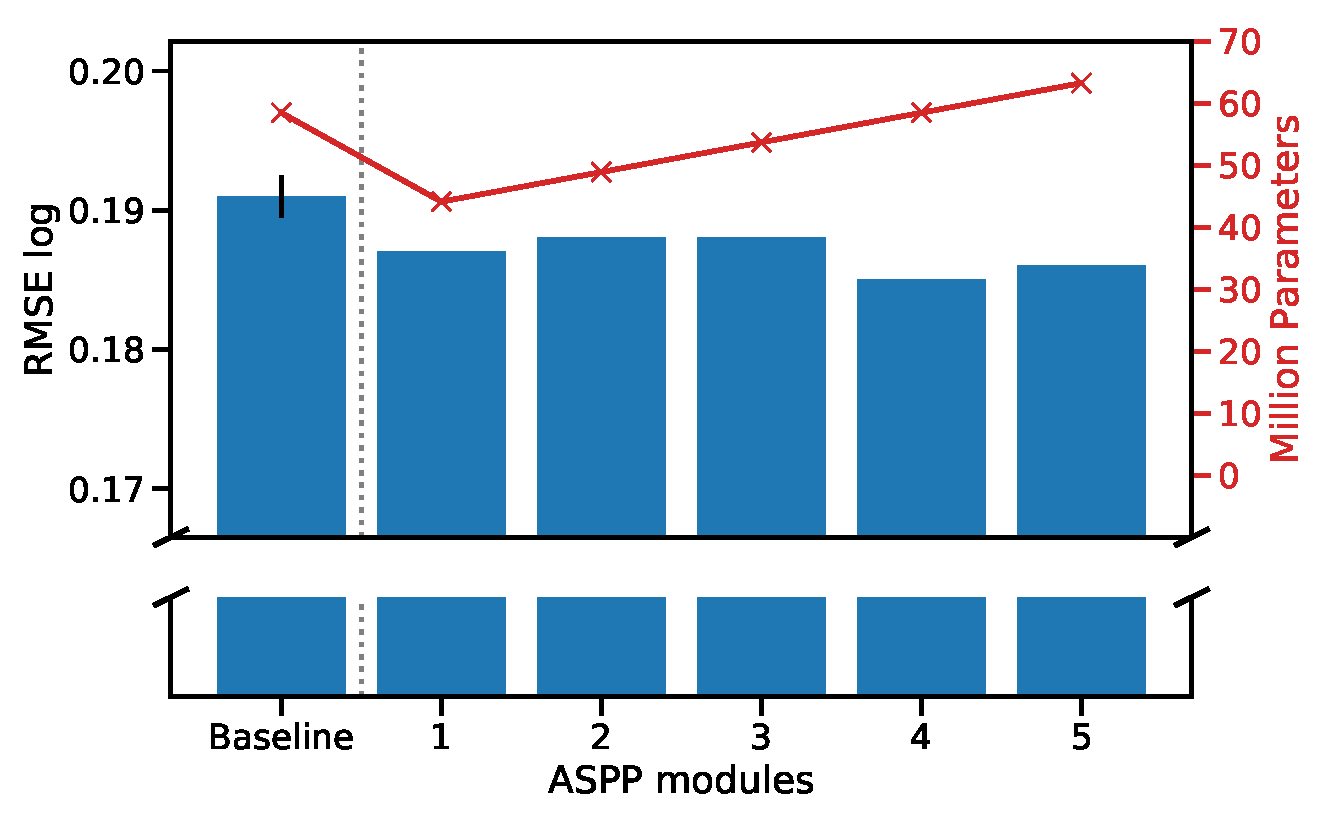
\includegraphics[width=1.0\textwidth]{figures/results/experiment2_RMSE log.pdf}
\end{frame}

\begin{frame}[c]{\subsecname: Atrous Rates (\% inliers 1)}
  \centering
  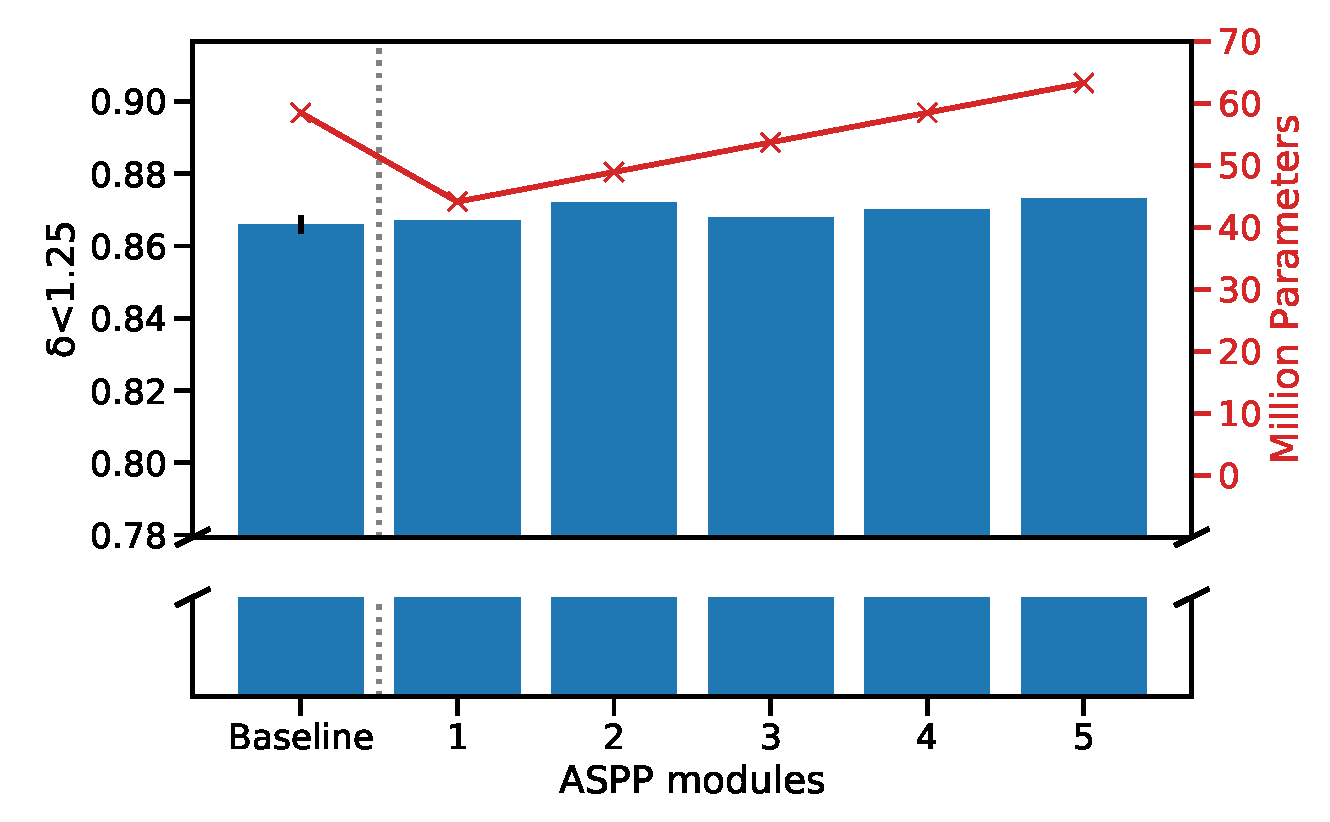
\includegraphics[width=1.0\textwidth]{figures/results/experiment2_d-125.pdf}
\end{frame}

\begin{frame}[c]{\subsecname: Atrous Rates (\% inliers 2)}
  \centering
  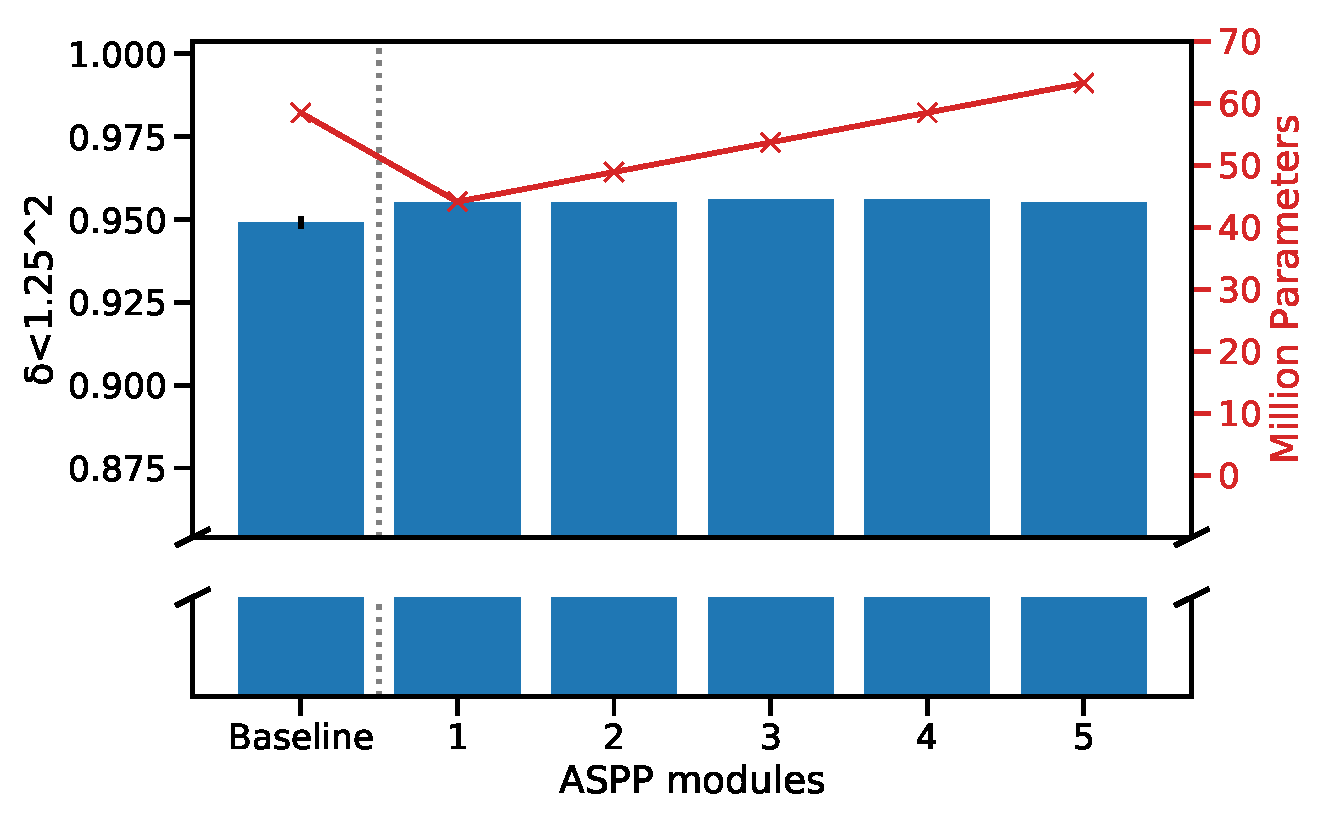
\includegraphics[width=1.0\textwidth]{figures/results/experiment2_d-125^2.pdf}
\end{frame}

\begin{frame}[c]{\subsecname: Atrous Rates (\% inliers 3)}
  \centering
  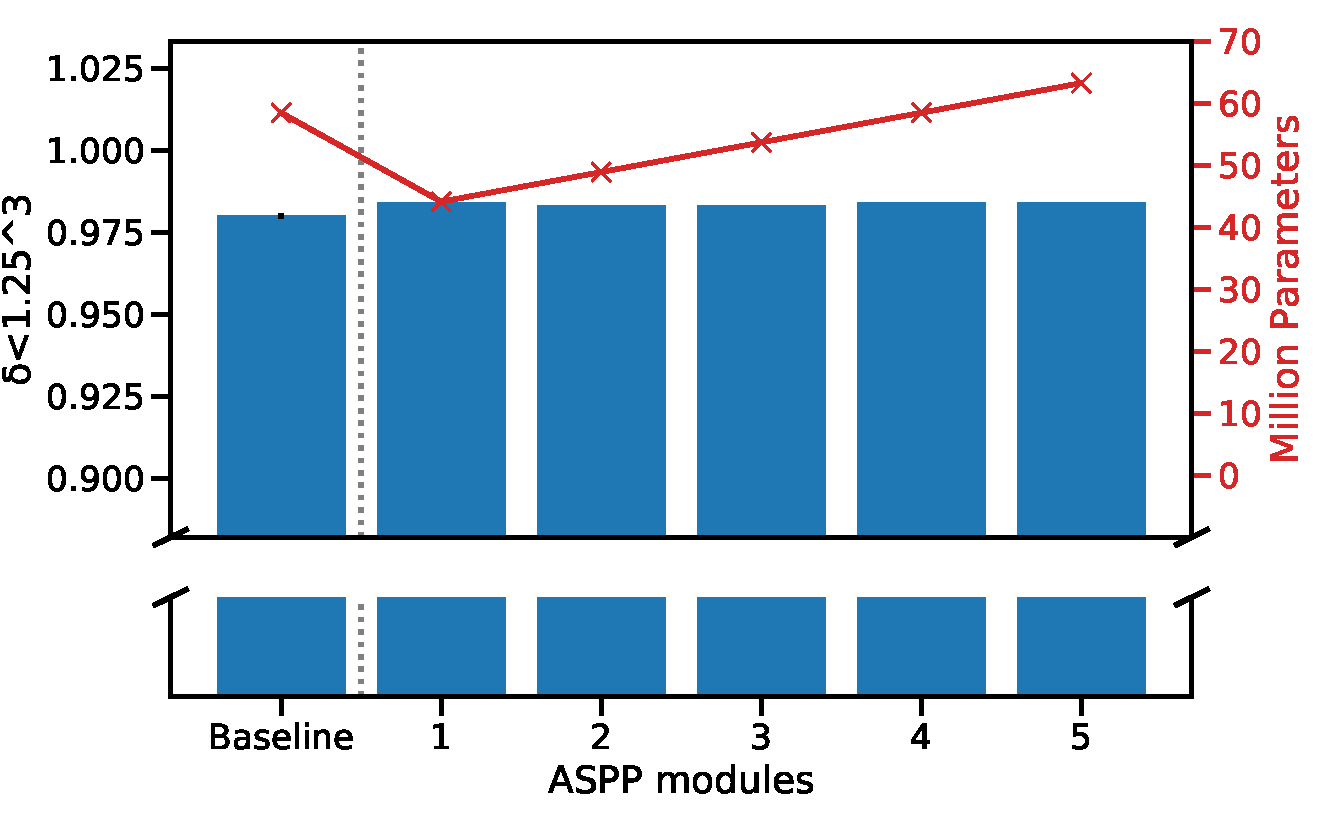
\includegraphics[width=1.0\textwidth]{figures/results/experiment2_d-125^3.pdf}
\end{frame}


\begin{frame}[c]{\subsecname: Output Stride Comparison}
  \centering
  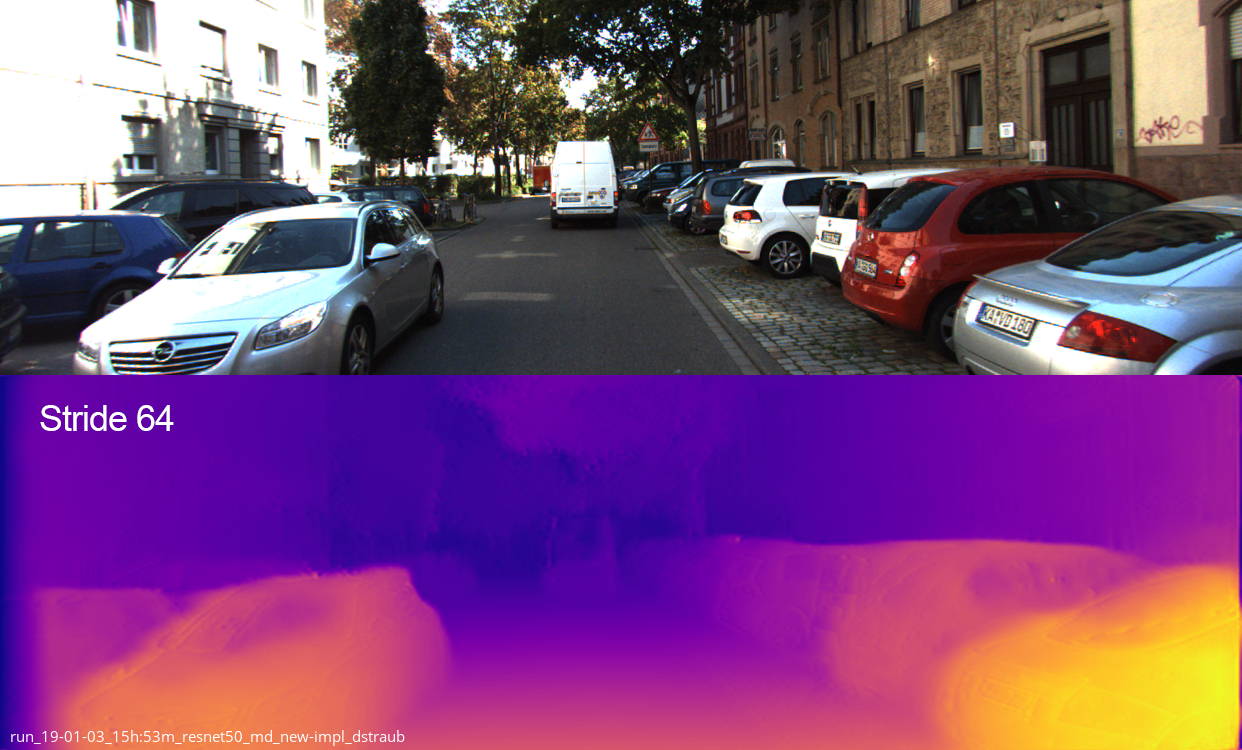
\includegraphics[width=1.0\textwidth]{figures/images/stridecomparison_001.png}
\end{frame}

\begin{frame}[c]{\subsecname: Output Stride Comparison}
  \centering
  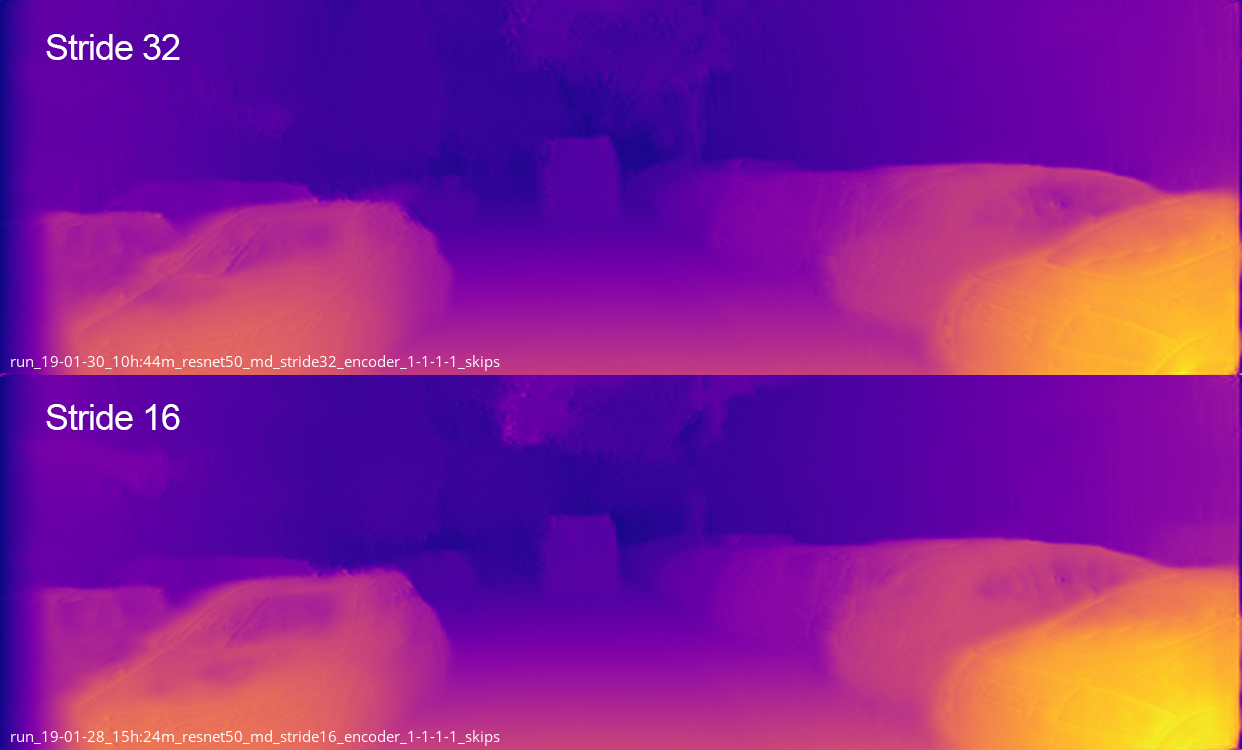
\includegraphics[width=1.0\textwidth]{figures/images/stridecomparison_002.png}
\end{frame}

\begin{frame}[c]{\subsecname: ASPP vs. no ASPP (without Skip Connections)}
\centering
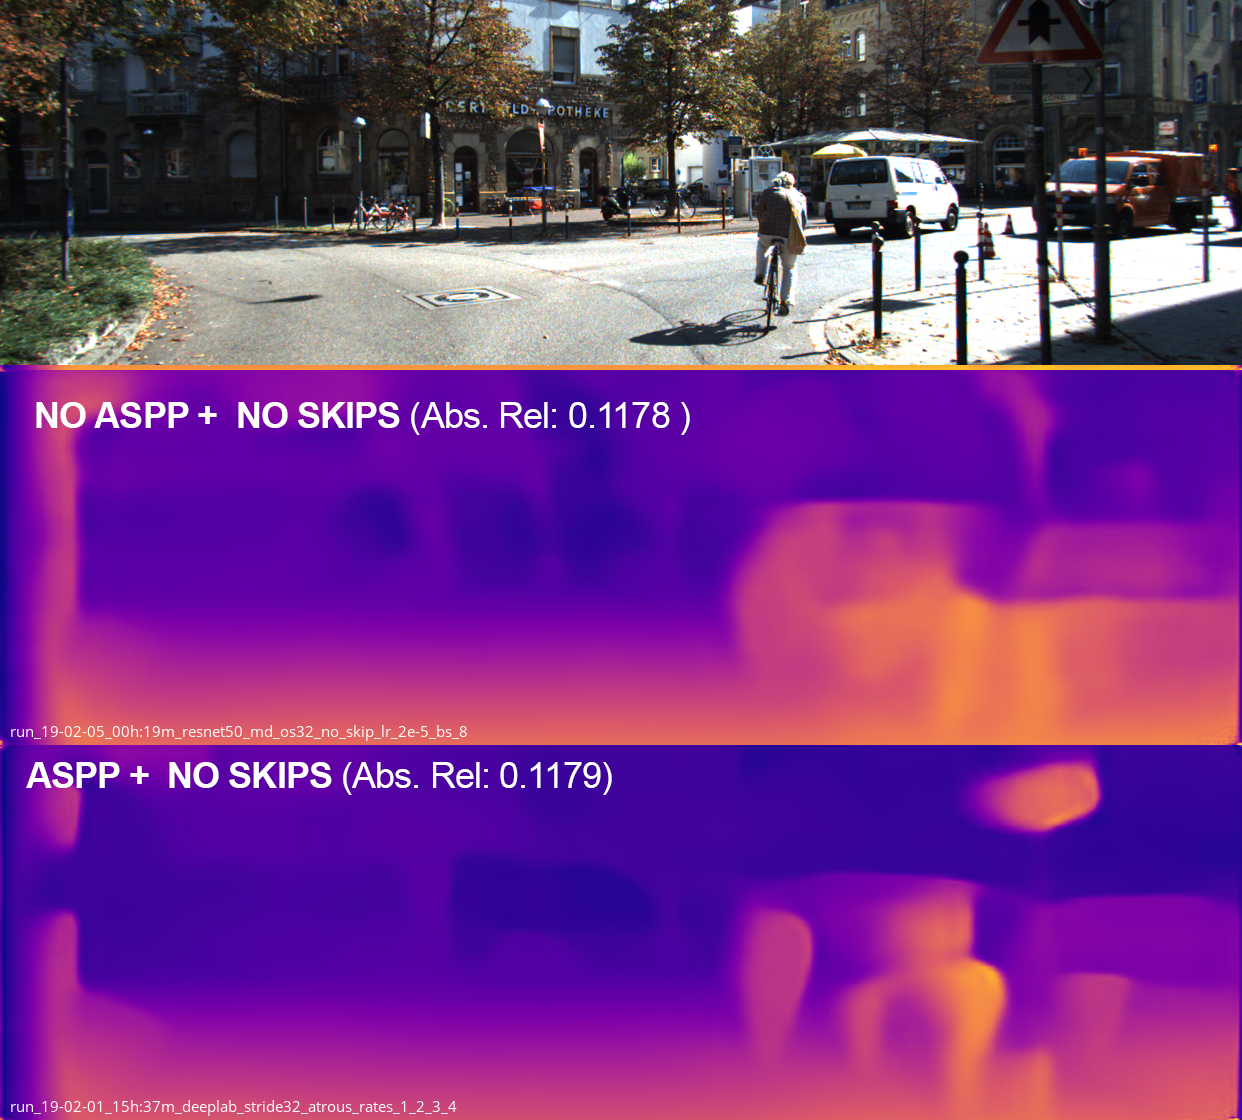
\includegraphics[width=0.7\textwidth]{figures/images/skipsvsnoskips2_error.png}
\end{frame}




